\chapter{Deriving a dynamical model of the actuators and combining it with the Simulink Model of chapter 2.2}\label{chapter:2}
\vspace{-0.25cm}
Responsible: \textit{Sophie Sepp}


\ \\

In task 2 a dynamical model of the actuators is derived and the Simulink model of task 1.ii is enhanced with the actuator models. The robotic arm LWA 4P has six brushless DC motors which are modelled in Simulink and combined with the Simulink model of task 1. The modelling of the motor is hereby divided by the electrical part of the motor equations and the dynamical part of the motor equations.

\section{Deriving a dynamical model of the actuators }


\subsection{Theoretical background: DC motor}
A DC-motor works on the principle that a current-carrying conductor in a magnetic field experiences a force, which can be expressed as the product of magnetic flux and the current in the conductor. It consists of a fixed stator, which provides a constant magnetic field and a armature part, which is a rotor that rotates inside the stator and is a simple coil. The armature is connected to a DC power source through a pair of commutator rings. The current that flows through the coil induces a electromagnetic force on it according to the Lorentz force, which causes the coil to rotate. Thus the commutator rings connect with the  power source of opposite polarity. As a result, on the left side electricity flows away while on the right side, electricity flows towards. Thus the torque action is in the same direction throughout the motion, which is the reason why the coil continues rotating. 
A characteristical aspect of DC motors is the production of back emf. A rotating loop in a magnetic field produces an emf according to the principle of electromagnetic induction, which are in this case the armature loops. So an internal emf will be induced, that opposes the applied input voltage. 
\begin{figure}[htsb]
  \centering
  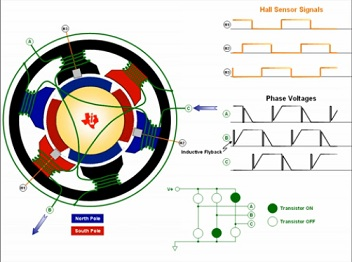
\includegraphics{figures/DC-motor.jpg}
  \caption{DC motor.}
\end{figure}




\clearpage


\subsection{Equations describing DC motor}

 Electrical part of the motor equations:

\begin{figure}[htsb]
  \centering
  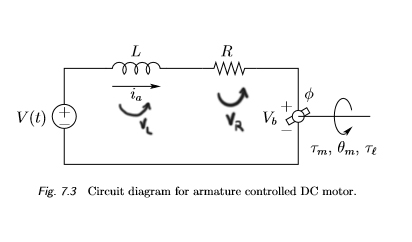
\includegraphics{figures/Circuit diagram for armature controlled DC motor.jpg}
  \caption{Circuit diagram for armature controlled DC motor.}
\end{figure}

V(t): Applied voltage\\
L: Armature self inductance\\
R: Armature resistence\\
\(V_{b}\): Back emf constant\\
\(\theta_{m}\): mechanical rotor angle\\
\(\tau_{m}\): generated torque\\
\(\tau_{l}\): load torque\\




\ \\
The voltage Vl and Vr can be computed in the following way: \\

\(V_{L}\) = \(L \cdot  \(\frac{di}{dt}\) \) \\

\(V_{R}\) = \(R \cdot i \) 



\clearpage

The electrical part of the motor can be computed by the sum of  Vl, Vr and the back emf. \\


\(V_{t}\)(t) = \(L \cdot \frac{di}{dt} \)+\(R \cdot i(t) \) + \(V_{emf}\) \\


The back (induced) electromotive force Vemf is proportional to the angular velocity ω(t) seen at the shaft.  Vb, the emf constant, also depends on certain physical properties of the motor. \\

\(V_{emf}\)(t) = \(\(V_{b}\) \cdot \omega(t) \) \\

The mechanical part of the motor equations is derived using Newton's law:  \\



\(J \cdot \(\frac{d\omega}{dt}\)  \)= \(\sum \limits_{i=1}^n \(\tau_i\)=\(- \(V_b\) \cdot \omega(t) \) + \(\(K_m\) \cdot i(t) \)  \\

The inertial load J times the derivative of angular rate equals the sum of all the torques about the motor shaft and can be expressed by the sum of the induced current i times the torque constant Km and the negative product of the back emf constant Kb and the angular velocity ω.

Moreover, the torque u seen at the shaft of the motor is proportional to the current i and can be expressed as the product of the current i and the torque constant Km, which is related to physical properties of the motor, such as magnetic field strength. \\


u(t) = \(\(K_m\) \cdot i(t) \)




